% Copyright 2004 by Till Tantau <tantau@users.sourceforge.net>.
%
% In principle, this file can be redistributed and/or modified under
% the terms of the GNU Public License, version 2.
%
% However, this file is supposed to be a template to be modified
% for your own needs. For this reason, if you use this file as a
% template and not specifically distribute it as part of a another
% package/program, I grant the extra permission to freely copy and
% modify this file as you see fit and even to delete this copyright
% notice. 

\documentclass{beamer}

% There are many different themes available for Beamer. A comprehensive
% list with examples is given here:
% http://deic.uab.es/~iblanes/beamer_gallery/index_by_theme.html
% You can uncomment the themes below if you would like to use a different
% one:
%\usetheme{AnnArbor}
%\usetheme{Antibes}
%\usetheme{Bergen}
%\usetheme{Berkeley}
%\usetheme{Berlin}
%\usetheme{Boadilla}
%\usetheme{boxes}
%\usetheme{CambridgeUS}
%\usetheme{Copenhagen}
%\usetheme{Darmstadt}
%\usetheme{default}
%\usetheme{Frankfurt}
%\usetheme{Goettingen}
%\usetheme{Hannover}
%\usetheme{Ilmenau}
%\usetheme{JuanLesPins}
%\usetheme{Luebeck}
\usetheme{Madrid}
%\usetheme{Malmoe}
%\usetheme{Marburg}
%\usetheme{Montpellier}
%\usetheme{PaloAlto}
%\usetheme{Pittsburgh}
%\usetheme{Rochester}
%\usetheme{Singapore}
%\usetheme{Szeged}
%\usetheme{Warsaw}


% Customize Warsaw color 
\setbeamercolor*{palette primary}{use=structure,fg=white,bg=red!50!black}
\setbeamercolor*{palette secondary}{use=structure,fg=white,bg=red!60!black}
\setbeamercolor*{palette tertiary}{use=structure,fg=white,bg=red!70!black}

% Customize Warsaw block title and background colors
\setbeamercolor{block title}{bg=red!50!black,fg=white}


% List your packages here

\usepackage[colorinlistoftodos]{todonotes}


\title[DC Motor Integration]{DC Motor Integration in BEMOSS}

% % A subtitle is optional and this may be deleted
% \subtitle{Product Proposal}

\author[B.~Lauer]{Brian~Lauer\\\and
Advisor: Dr. Suruz Miah}
% - Give the names in the same order as the appear in the paper.
% - Use the \inst{?} command only if the authors have different
%   affiliation.

\institute[Bradley University] % (optional, but mostly needed)
{
  Department of Electrical and Computer Engineering\\
  Bradley University\\
  1501 W. Bradley Avenue\\
  Peoria, IL, 61625, USA
}
% - Use the \inst command only if there are several affiliations.
% - Keep it simple, no one is interested in your street address.

\date[August~16,~2019]{Friday, August~14,~2019}
% - Either use conference name or its abbreviation.
% - Not really informative to the audience, more for people (including
%   yourself) who are reading the slides online

\logo{\hfill\href{http://www.bradley.edu}{
\includegraphics[width=0.75cm]{figs/logoBU1-Print}}}  % place logo in every page 


\subject{Building Energy Management}
% This is only inserted into the PDF information catalog. Can be left
% out. 

% If you have a file called "university-logo-filename.xxx", where xxx
% is a graphic format that can be processed by latex or pdflatex,
% resp., then you can add a logo as follows:

% \pgfdeclareimage[height=0.5cm]{university-logo}{university-logo-filename}
% \logo{\pgfuseimage{university-logo}}

% Delete this, if you do not want the table of contents to pop up at
% the beginning of each subsection:
% Let's get started
\begin{document}

\begin{frame}
  \titlepage
\end{frame}

\begin{frame}{Outline}
  \tableofcontents
  % You might wish to add the option [pausesections]
\end{frame}
%----------------------------------

\section{Device API Traslator}


\begin{frame}{Device API Translator}{}
\begin{figure}
\includegraphics[scale=0.35]{figs/Architecture35.png}
\caption{Courtesy of BEMOSS developer resources}
\end{figure}
\end{frame}

\section{Steps in adding device API}

\begin{frame}{Steps in adding device API}{}
\begin{block}{Methods to implement}
\begin{itemize}
	\item \texttt{API\_info} returns list of supported device attributes (\texttt{device\_model}, \texttt{vendor\_name}, \texttt{html\_template}, \texttt{chart\_template} etc.)
	\item \texttt{dashboard\_view} returns parameters of device to be shown on the BEMOSS dashboard
	\item \texttt{ontology} maps parameters from device to BEMOSS parameters
	\item \texttt{discover} is called by the device discovery agent and returns attributes of discovered devices
	\item \texttt{getDataFromDevice} returns dictionary of device data
	\item \texttt{identifyDevice} visually identifies the device, triggered by web UI and sends message to control agent
	\item \texttt{setDeviceStatus} sends control commands to device
\end{itemize}
\end{block}
\end{frame}

\begin{frame}{Steps in adding device API}{}
\begin{block}{Methods in motor API}
\begin{itemize}
	\item \texttt{argsToPi} uses ssh to run \texttt{XBEEcontrol.py} with arguments to control motor and retrieve data
	\item \texttt{toggleDeviceStatus} queries the device for on/off status then changes settings of the motor, uses \texttt{getDataFromDevice} and \texttt{setDeviceStatus}
\end{itemize}
\end{block}
\end{frame}

\section{Steps in adding new device type}
\begin{frame}{Steps in adding new device type}{}
\begin{block}{Steps}
\begin{itemize}
\item Select a device type id (1, 2, 3, 4 and 7 are reserved)
\item Register new device type in BEMOSS db by updating \texttt{PROJECT\_DIR/Web\_Server/defaultDB.py} then running the script
\item Update \texttt{discover\_devices} function in \texttt{Web\_Server/webapps/discovery/views.py}
\item Add widget for new device in \texttt{Web\_Server/webapps/
discovery/templates/discovery/manual\_discovery.html}
\item Update \texttt{Web\_Server/static/app\_js/discovery.js} with code to enable use of the "Set all to 'Approved'" button in the Device Discovery page
\end{itemize}
\end{block}
\end{frame}

\begin{frame}{Steps in adding new device type}{}
\begin{figure}
\includegraphics[scale=0.25]{figs/motorapproval.png}
\caption{Device discovery page}
\end{figure}
\end{frame}

\section{Problems Fixed}
\begin{frame}{Problems Fixed}{}
\begin{figure}
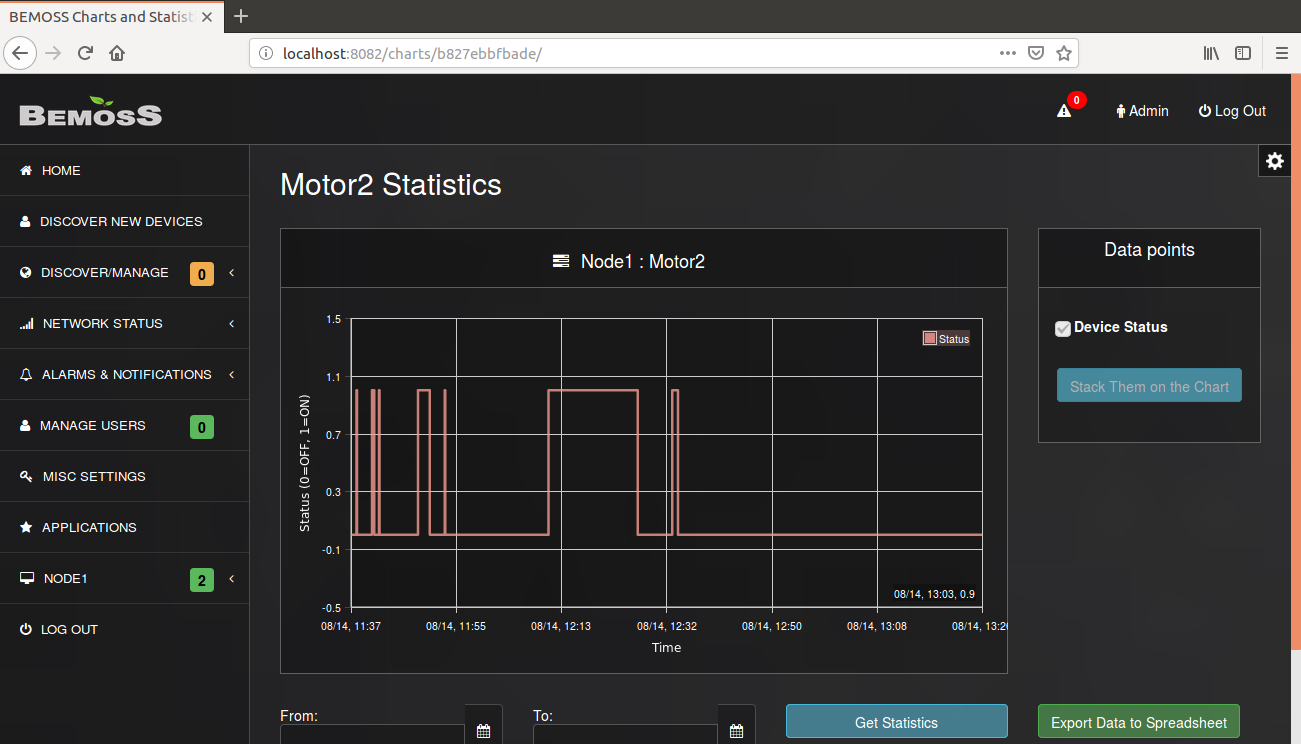
\includegraphics[scale=0.25]{figs/motorchart.png}
\caption{Fully functional jQuery plot}
\end{figure}
\end{frame}

\section{Additions}
\begin{frame}{Additions}{}
\begin{block}{ssh keys}
\begin{itemize}
\item \texttt{ssh-keygen} generates a public and private key
\item Public key copied to RPi, private key kept on host machine
\item More secure than using password
\item \url{https://www.raspberrypi.org/documentation/remote-access/ssh/passwordless.md}
\end{itemize}
\end{block}
\end{frame}
%----------------------------------

\section{Priorities}
\begin{frame}{Priorities}{}
\begin{itemize}
\item Write paper
\item Speed control algorithm
\item Still looking for new device
\end{itemize}
\end{frame}

% You can reveal the parts of a slide one at a time
% with the \pause command:
%\begin{frame}{Second Slide Title}
%  \begin{itemize}
%  \item {
%    First item.
%    \pause % The slide will pause after showing the first item
%  }
  %\item {   
  %  Second item.
 % }
  % You can also specify when the content should appear
  % by using <n->:
 % \item<3-> {
 %   Third item.
 % }
%  \item<4-> {
%    Fourth item.
 % }
  % or you can use the \uncover command to reveal general
  % content (not just \items):
%  \item<5-> {
%    Fifth item. \uncover<6->{Extra text in the fifth item.}
%  }
%  \end{itemize}
%\end{frame}

%\section{Second Main Section}

%\subsection{Another Subsection}

%\begin{frame}{Blocks}
%\begin{block}{Block Title}
%You can also highlight sections of your %presentation in a block, with it's own %title
%\end{block}
%\begin{theorem}
%There are separate environments for %theorems, examples, definitions and proofs.
%\end{theorem}
%\begin{example}
%Here is an example of an example block.
%\end{example}
%\end{frame}

% Placing a * after \section means it will not show in the
% outline or table of contents.

\end{document}



%%% Local Variables:
%%% mode: latex
%%% TeX-master: t
%%% End:
